\documentclass[12pt, a4paper, oneside]{report}

\usepackage[utf8]{inputenc}
\usepackage[T1]{fontenc}
\usepackage[polish]{babel}
\usepackage{setspace}
\usepackage{titlesec}
\usepackage[pdftex]{graphicx}     
\usepackage{float}


\titleformat{\chapter}[block]{\Large\bfseries\filcenter}{}{1em}{}
\titleformat{\section}[block]{\large\bfseries}{}{1em}{}
\usepackage[font={small, it}]{caption}


\title{\Huge \textbf{Przykłady złych interfejsów w rzeczywistości}\\\,\\
       \Large Komunikacja człowiek-komputer 2019\\
       Zadanie 1}
\date{\today}
\author{Jakub Grobelny, Jakub Remiszewski, Kacper Bukowiec}

\setstretch{1.4}

\begin{document}

\begin{titlepage}
    \maketitle
    \thispagestyle{empty}
\end{titlepage}

\renewcommand*\thesubsection{\arabic{section}}


\chapter*{SKOS - System komunikacji na odległość ze studentami UWr}

Jedną ze stron internetowych, z jaką regularnie styczność ma każdy student
informatyki na naszej uczelni, jest tak zwany SKOS. Niestety w kwestii wygody
użytkowania i czytelności jest to system, który pozostawia wiele do życzenia, 
co zapewniło mu miejsce w tym raporcie. \\

\begin{figure}[H]
    \centering
    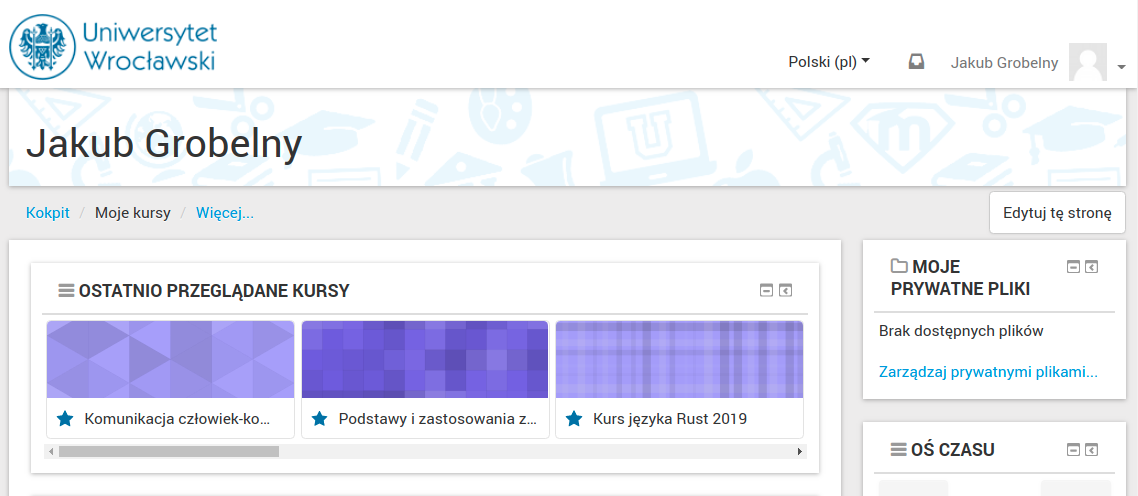
\includegraphics[scale=0.30]{./img/skos_header.png}
    \caption{Nagłówek witryny SKOS.}
    \label{figure:skos-header}
\end{figure}

Pierwszym miejscem, w jakim pojawimy się po zalogowaniu, jest strona
,,kokpit'' gdzie mamy dostęp do wszystkich kursów, w których uczestniczymy.
Wyobraźmy sobie jednak sytuację, w której ktoś chciałby zapisać się na jakiś
kurs własnoręcznie. Pojawia się wówczas pytanie -- w jaki sposób można znaleźć
konkretny kurs? Okazuje się, że odpowiedź na nie nie jest taka oczywista jak
by się mogło wydawać. Na rysunku \ref{figure:skos-header} widzimy, że 
wyszukiwarka nie znajduje się tam, gdzie byśmy jej oczekiwali -- na samej górze 
strony. Możemy zaobserwować, że paska wyszukiwania nie znajdziemy nigdzie na tej 
stronie. Aby dostać się do wyszukiwarki  trzeba przenieść się na stronę główną
(o istnieniu której można nawet nie wiedzieć, gdyż nawet po kliknięciu w logo 
Uniwersytetu Wrocławskiego zostajemy zawsze przekierowani do ,,kokpitu'').

\begin{figure}
    \centering
    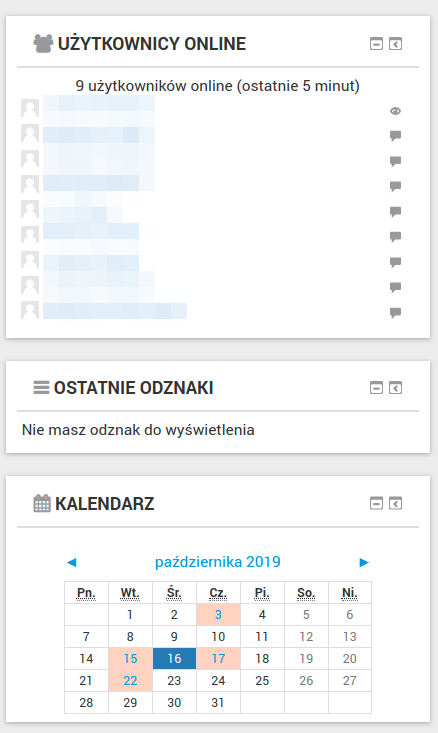
\includegraphics[scale=1.50]{./img/skos_side.png}
    \caption{Lista użytkowników online i kalendarz w witrynie SKOS; paska 
             wyszukiwania wciąż ani śladu.}
    \label{figure:skos-side}
\end{figure}

W celu dostania się na stronę główną, musimy odszukać panel zatytuowany 
,,nawigacja'', który (jakże by inaczej) położony jest na samym dole strony.
Panel ten widzimy na rysunku \ref{figure:skos-nav}.

\begin{figure}[H]
    \centering
    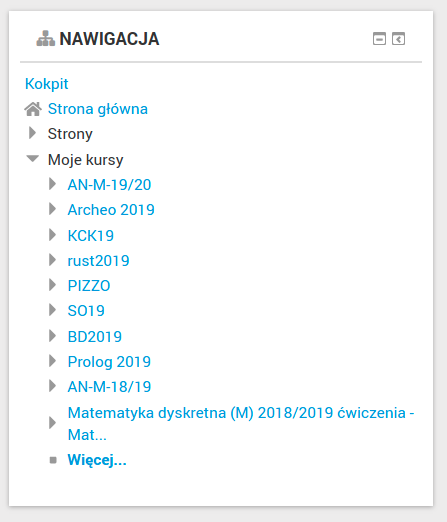
\includegraphics[scale=0.43]{./img/skos_nav.png}
    \caption{Skrzętnie ukryta przed użytkownikiem 
             ,,nawigacja'' w witrynie SKOS.}
    \label{figure:skos-nav}
\end{figure}

Strona główna (rysunek \ref{figure:skos-main}) tak właściwie powiela 
funkcjonalność ,,kokpitu'', gdyż również jest listą naszych kursów, która jest 
dodatkowo o wiele bardziej rozwlekła wertykalnie, co sprawia, że na raz widzimy 
na ekranie zaledwie kilka z nich. Gdy przewiniemy stronę na sam dół, naszym
oczom ukaże się upragniony pasek wyszukiwania (przedstawiony na rysunku \ref{figure:skos-search}).

Żeby znacznie poprawić ten interfejs wystarczyłoby przenieść wyszukiwarkę na 
dobrze widoczne miejsce w ,,kokpicie''.

\begin{figure}[H]
    \centering
    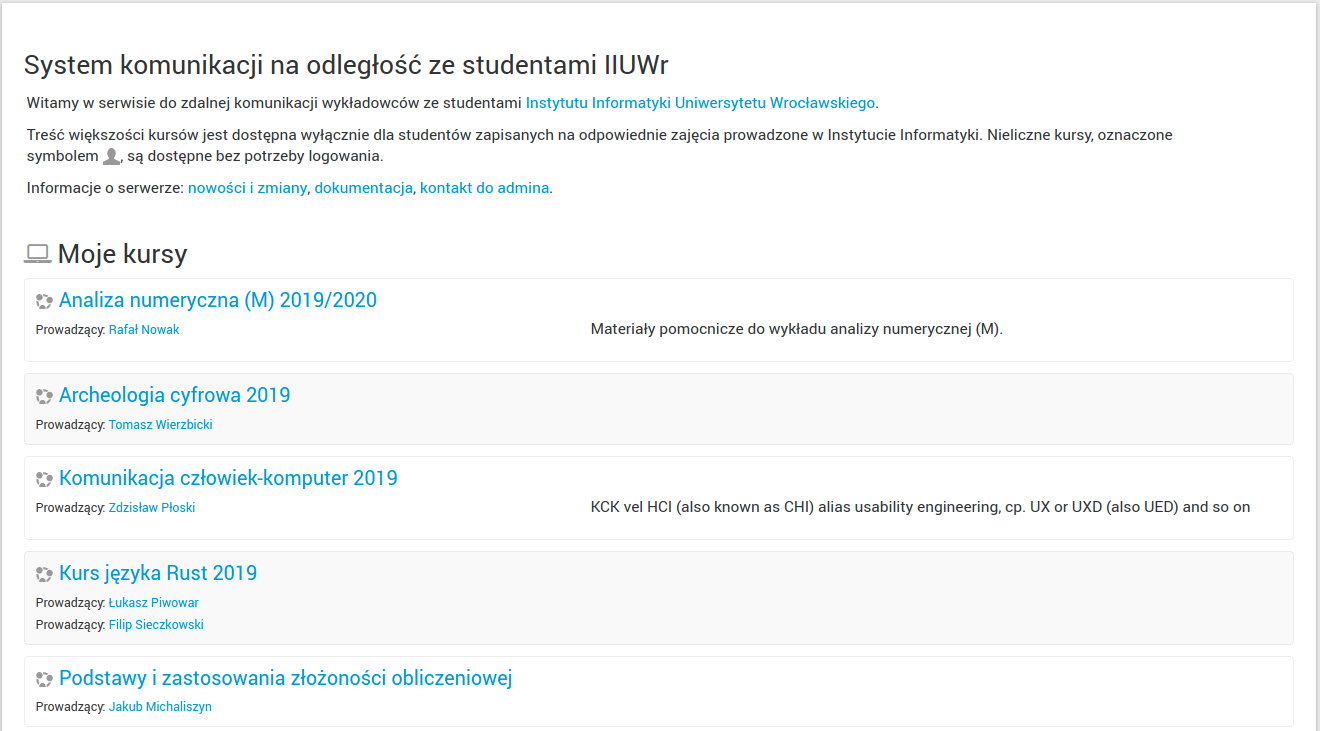
\includegraphics[scale=0.25]{./img/skos_main.png}
    \caption{Strona główna witryny SKOS.}
    \label{figure:skos-main}
\end{figure}


\begin{figure}[H]
    \centering
    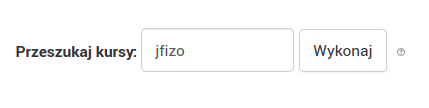
\includegraphics[scale=0.8]{./img/skos_search.png}
    \caption{Nieoficjalny mistrz witryny SKOS w zabawie w chowanego.}
    \label{figure:skos-search}
\end{figure}


Przejdźmy teraz do miejsca gdzie wszystko się rozpoczęło -- do ,,kokpitu''.
Pierwsze co możemy zauważyć, to to, że grafiki wyświetlane przy nazwach
przedmiotów potrzebują chwili aby się załadować co bywa frustrujące, gdyż
trzeba poczekać nawet do sekundy.

Przyjrzyjmy się teraz dokładniej ,,przeglądowi kursów'', który jest centralną
częscią ,,kokpitu''. Kursy można sortować według nazwy bądź czasu ostatniego
przeglądania. Da się je również filtrować według kategorii takich jak 
,,aktualne'' (prowadzący niestety często zapominają o zakończeniu kursu w
SKOSie więc zostaje on w tej kategorii na wieczność) lub ,,oznaczone gwiazdką''.
W porównaniu do strony głównej mamy do czynienia z o wiele gęstszym ułożeniem
przedmiotów (chyba, że korzystamy na przykład z telefonu -- 
rysunek \ref{figure:skos-mobile}). Nie znaczy to bynajmniej, że jest to
czytelne. Większość kursów korzysta z domyślnej grafiki przez co trudno jest
je od siebie od razu odróżnić. Niestety uwagę przykuwają właśnie te obrazki a
nie znajdujący się pod nimi tekst przez co szybkie poruszanie się między kursami
wymaga przyzwyczajenia.

Oprócz kafelków istnieje opcja wyświetlania w formie listy oraz 
,,podsumowania''. Oba te warianty są do siebie bardzo podobne (podsumowanie
w przeciwieństwie do listy zawiera obrazki oraz opisy kursów) i są wygodniejsze
niż domyślny widok.\\

\begin{figure}[H]
    \centering
    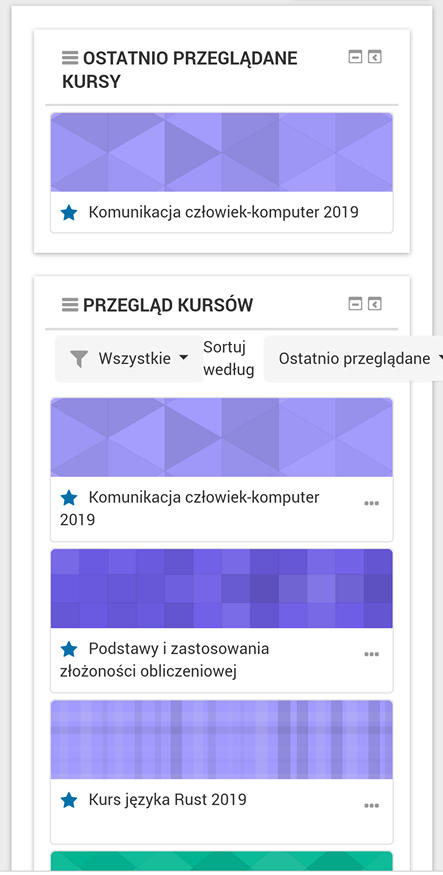
\includegraphics[scale=1.7]{./img/skos_mobile.png}
    \caption{Przegląd kursów witryny SKOS w wersji mobilnej. Widać, że grafiki
             nie pomagają odróżniać od siebie kursów a jedynie zajmują cenne
             miejsce.}
    \label{figure:skos-mobile}
\end{figure}


Podsumowując, głównymi wadami SKOSu są nieintuicyjnie rozmieszczone elementy
oraz niewygodny sposób prezentacji listy kursów użytkownikowi. Wiele elementów
interfejsu (takie jak ,,użytkownicy online'') jest na tyle mało użytecznych, że
mogłyby zostać ukryte co stworzyłoby więcej miejsca dla faktycznej treści.
Ponadto mamy do czynienia z rażącą redundancją -- zaraz nad panelem 
,,nadchodzące wydarzenia'' znajduje się kalendarz, który zawiera dokładnie
te same informacje (przedstawione w czytelniejszy sposób), zaś strona główna
pełni te same funkcje co ,,kokpit'' lecz z niewiadomych przyczyn tylko tam 
znajdziemy wyszukiwarkę kursów.


\begin{figure}
    \centering
    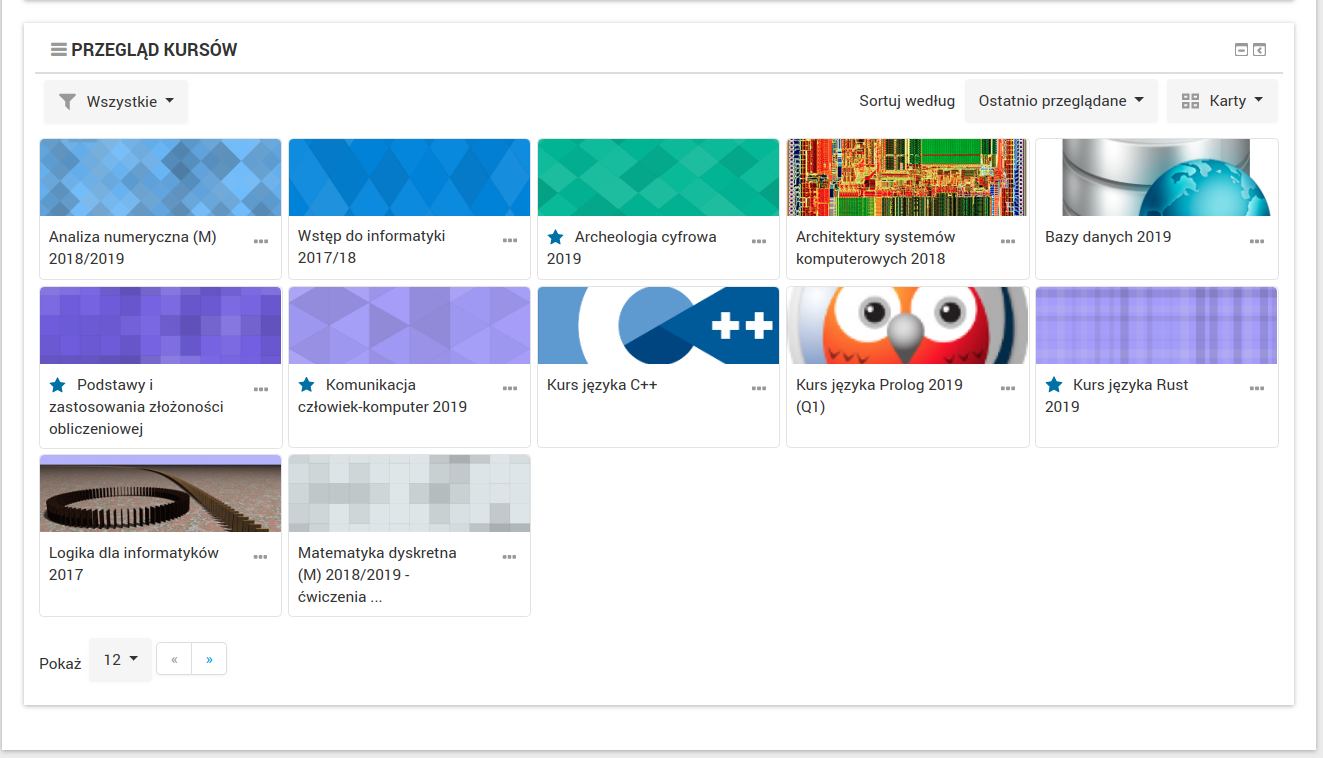
\includegraphics[scale=1.3]{./img/skos_view.png}
    \caption{Przegląd kursów witryny SKOS na komputerze.}
    \label{figure:skos-mobile}
\end{figure}


\end{document}
